
\section{Project description}
The purpose of the project work is to construct a pan and tilt system, for the set up shown in figure \ref{fig:pantilysystem}, so that it is possible to control the system from one or more user inputs for example a joystick, a keyboard, buttons or via commands from a computer. In addition the system should also give the user options for feedback of significant system parameters.

\begin{figure}[htb]
	\centering
	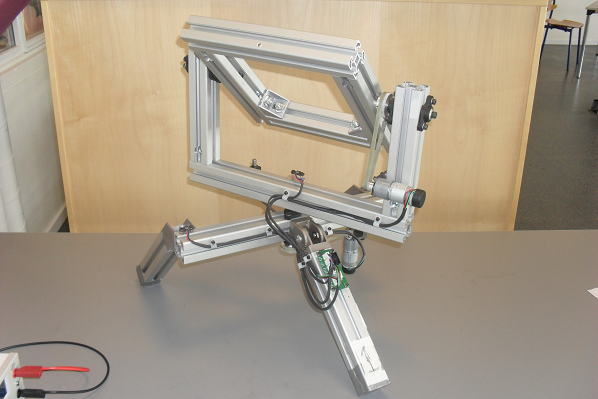
\includegraphics[width=\textwidth]{graphics/pantiltsystem.png} %trim=l b r t
	\caption{The given pan tilt system.}
	\label{fig:pantilysystem}
\end{figure}

This is to be prioritized in the project:
\begin{itemize}
\item A system analysis and modulation of the systems individual elements.
\item Analysis and design of the regulation loops in Matlab and Simulink.
\item Documentation of FPGA design and implementation.
\item Documentation of the microprocessor programs design and implementation, including division into tasks and selection of scheduling.
\item Test and verification of the system.
\end{itemize}

It is up to the project group to chose the regulator system and the regulator loops characteristics.

\section{Requirements}

The following conditions are set for the system:
\begin{itemize}
\item The controllers must be implemented on a microprocessor.
\item SPI must be used in communication between the microprocessor and the FPGA.
\item The FPGA must control the PWM signals to the motors.
\item The FPGA must be used to determine the motors position via the encoders.
\end{itemize}

\section{Overall System Design}

Thus the system will overall consist of four parts. As shown in figure \ref{fig:firstsystem} there is the psychical system \ref{sec:phsycicalsystem} connected with an FPGA \ref{sec:FPGA} which is connected with SPI to a microprocessor \ref{sec:microprocessor} which is connected to i/o devices \ref{sec:iodevices}.

\begin{figure}[htb]
	\centering
	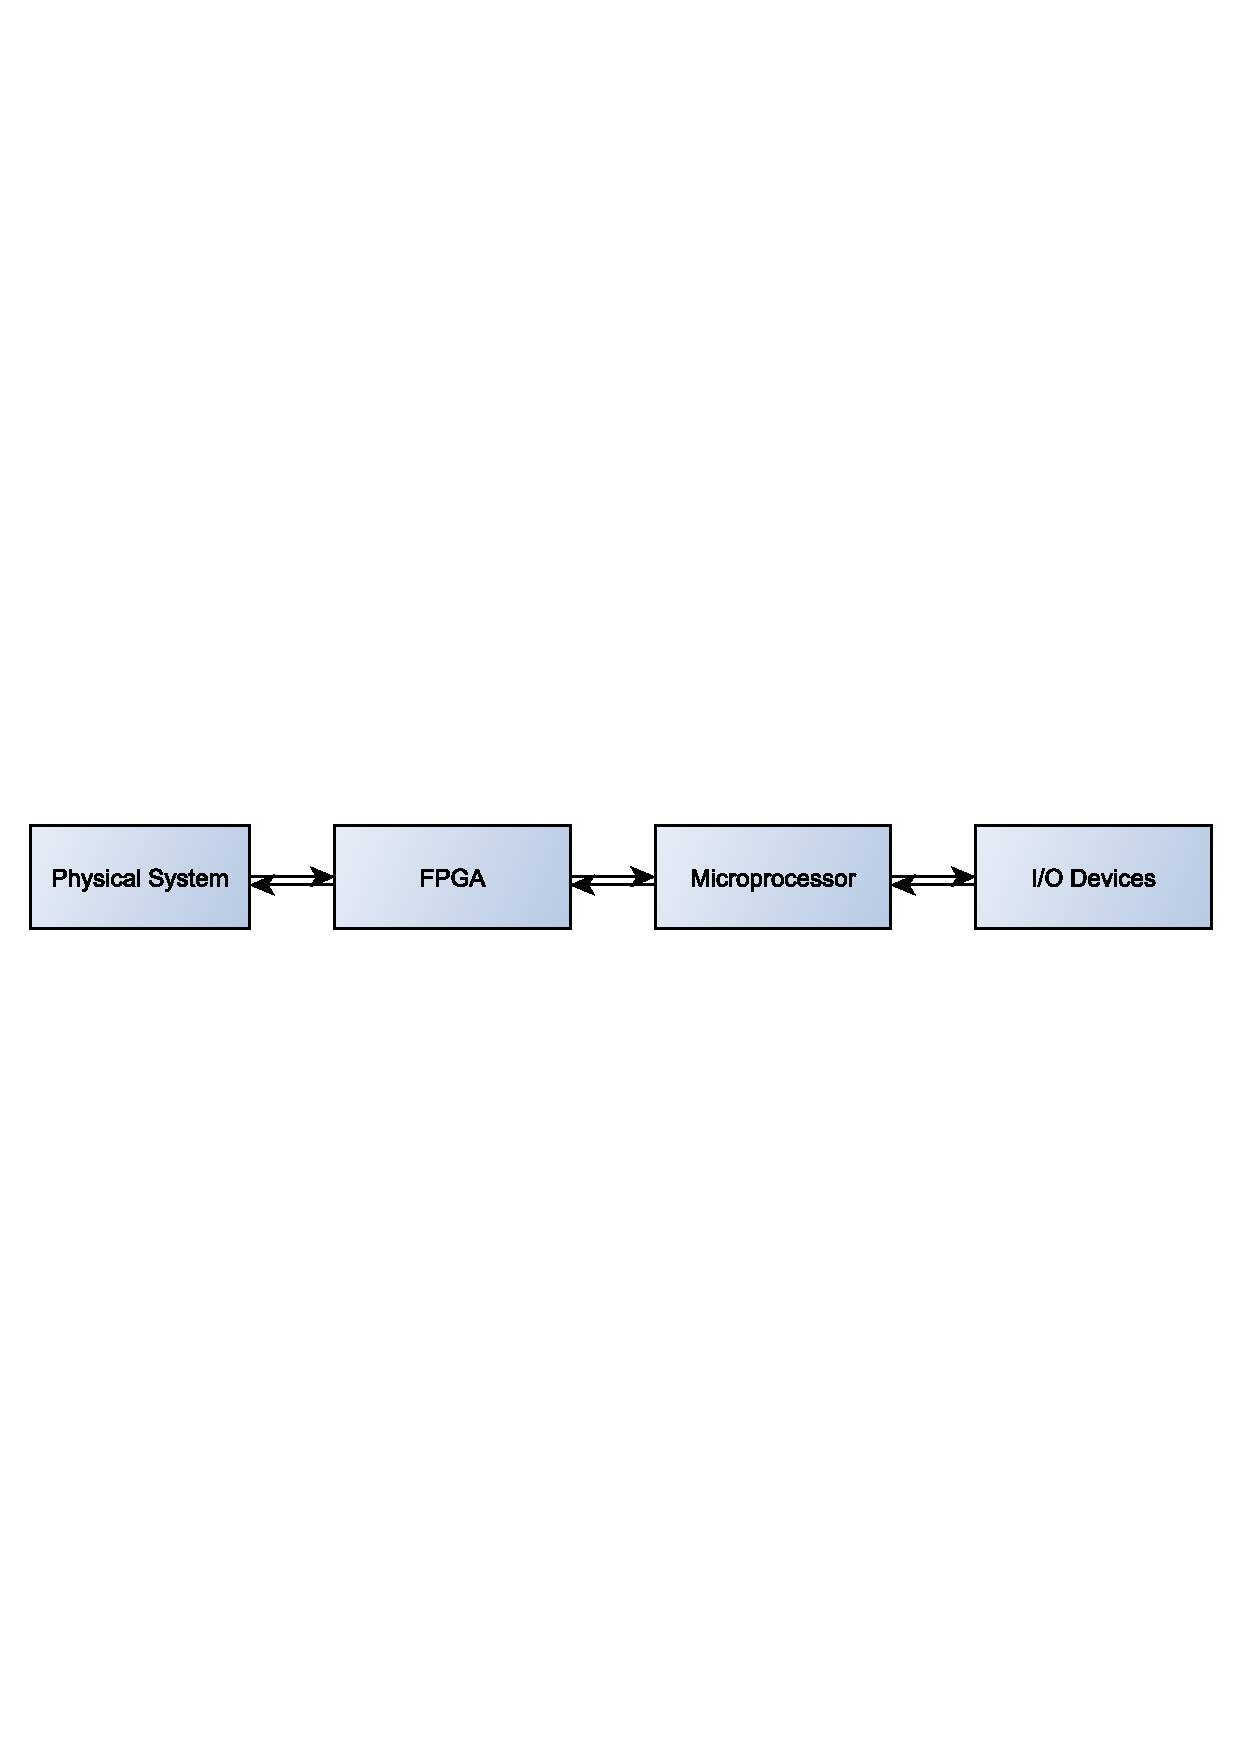
\includegraphics[scale=0.6,trim=400 380 400 380]{graphics/firstsystem} %trim=l b r t (can cut off from every side)
	\caption{Overall view of the system.}
	\label{fig:firstsystem}			% figure labels are of the form \label{fig:*}
\end{figure}

\section{The physical system}\label{sec:phsycicalsystem}

The physical system is provided for the project. It consist of a pan/tilt system driven by two EMG30 \cite{emg30} motors with inbuilt encoders. The motors are driven by an H-bridge \cite{hbridge} with 12 volt dc supply connected. Thus the system are controlled trough the H-bridge and output is collected by the encoders.

\begin{figure}[htb]
	\centering
	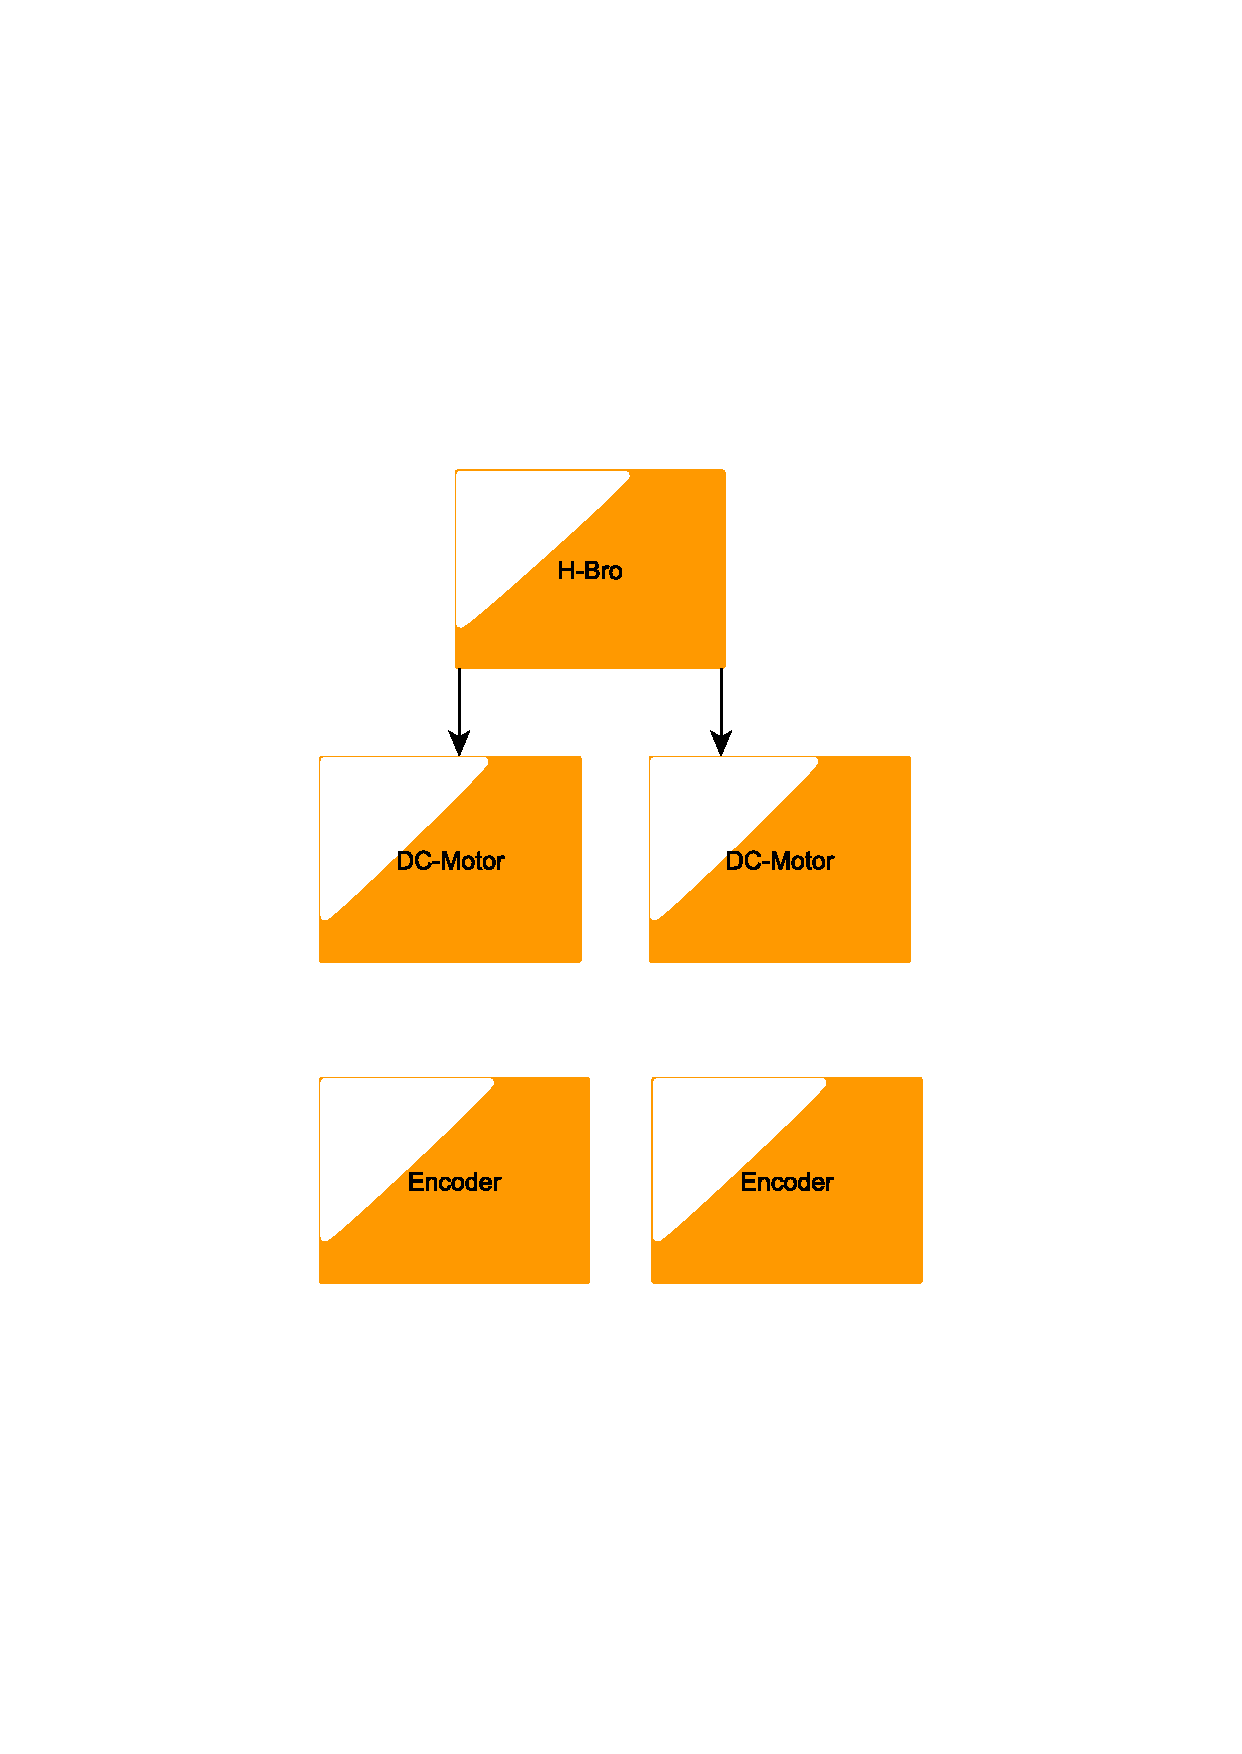
\includegraphics[scale=0.4,trim=200 200 200 200]{graphics/phsycicalsystem} %trim=l b r t (can cut off from every side)
	\caption{Set up of the physical system.}
	\label{fig:phsysicalsystem}			% figure labels are of the form \label{fig:*}
\end{figure}

\section{FPGA system}\label{sec:FPGA}

The FPGA is a Xilinx Nexys 2 board with a Spartan-3E chip on board. Multiple processes will have to run on the FPGA. It is controlling the motors, watching the encoders and communicating with the microprocessor. Thus the three main processes are the SPI communication, the motor PWM and the encoder. Both the PWM and encoder process are to run double because two motors are controlled. 

\begin{figure}[htb]
	\centering
	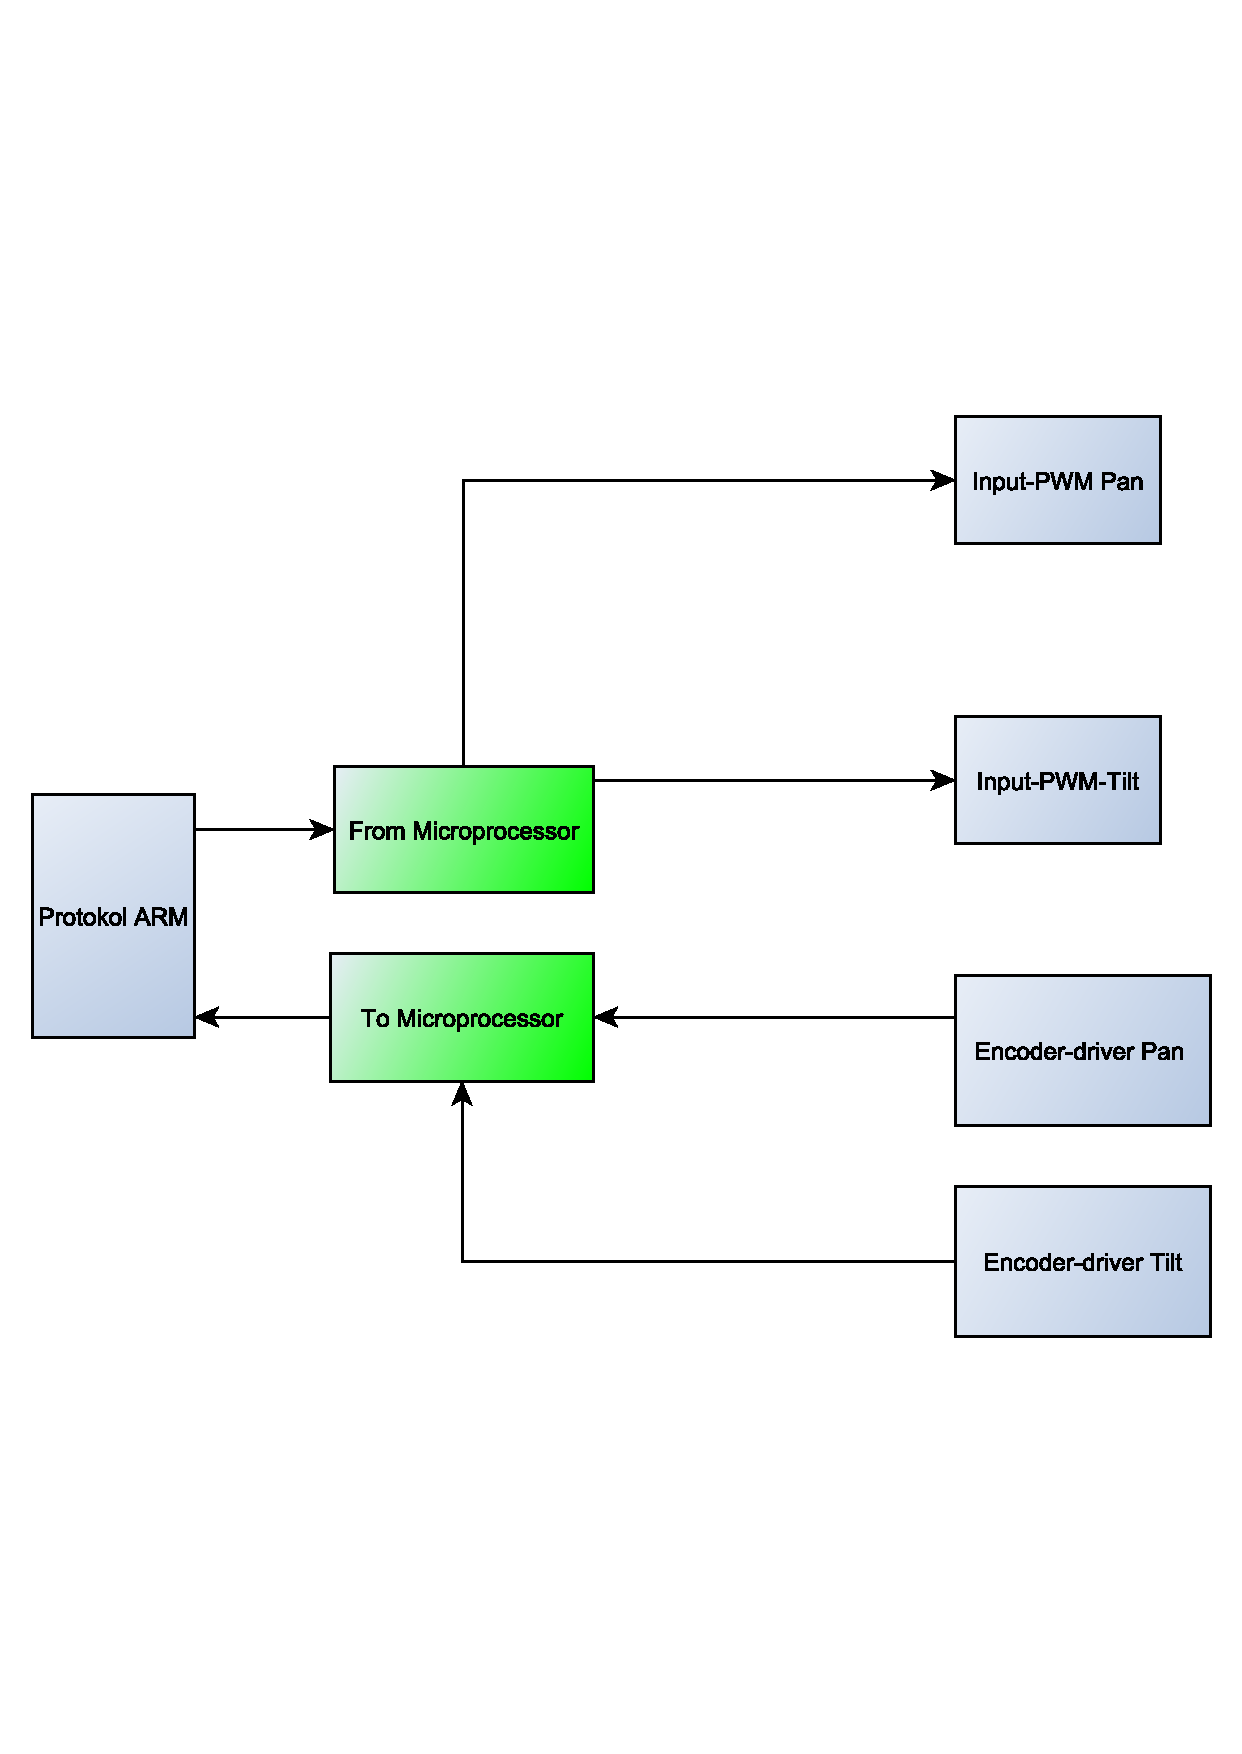
\includegraphics[scale=0.42,trim=200 200 200 200]{graphics/FPGA} %trim=l b r t (can cut off from every side)
	\caption{Setup of the FPGA processes.}
	\label{fig:FPGA}			% figure labels are of the form \label{fig:*}
\end{figure}

\section{Microprocessor}\label{sec:microprocessor}

The microprocessor is an ARM Cortex M3 mounted on a Stellaris LM3S6965 Evaluation Board. The microprocessor is both to run the control, the user interface\ref{chap:ui} and the communication with the SPI. By sharing the parameters between the tasks they have a standard interface and are all working with the same parameters as seen in  \ref{tab:parameters}. Because the microprocessor will run multiple tasks communicating with each other some sort of scheduler and intertask communication will be needed\ref{chap:os}.

\begin{figure}[htb]
	\centering
	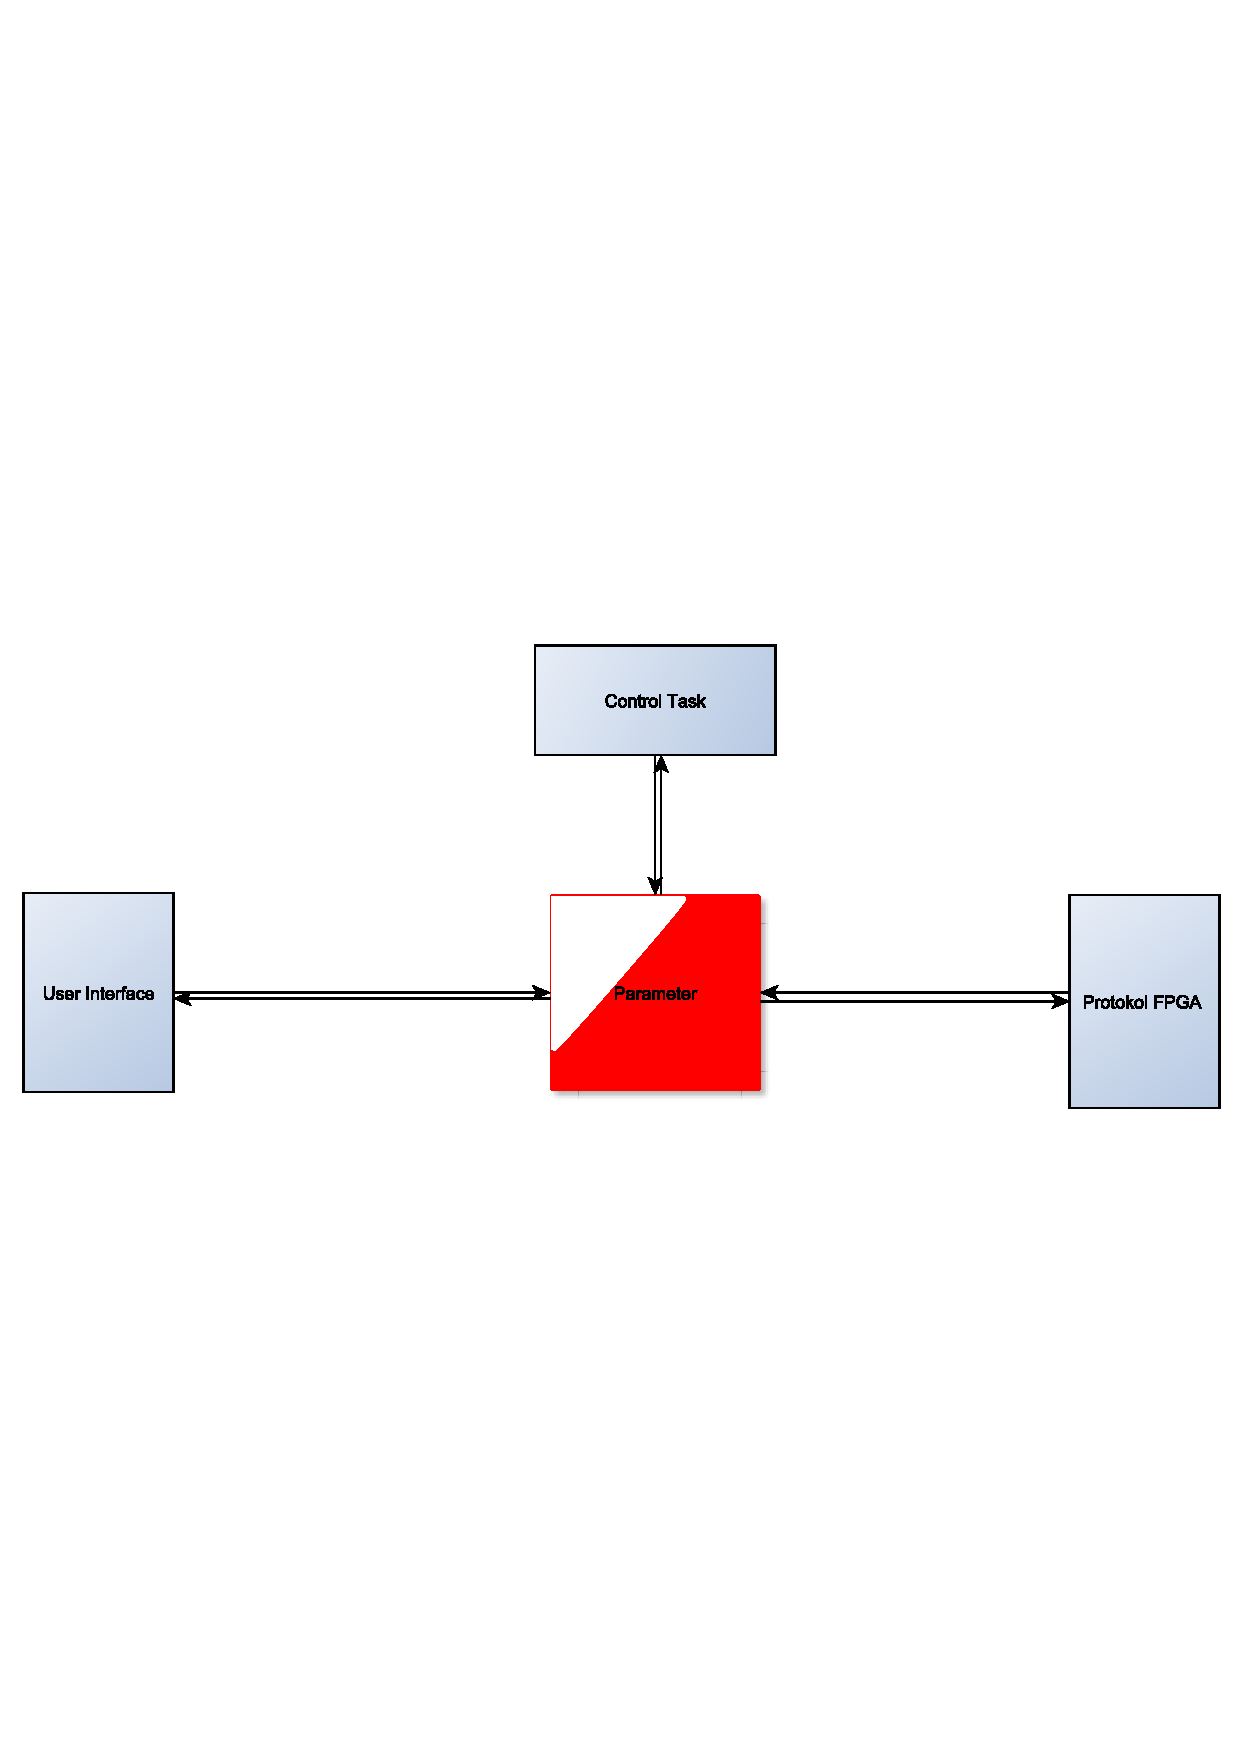
\includegraphics[scale=0.5,clip,trim=0 300 0 300]{graphics/microprocessor} %trim=l b r t (can cut off from every side)
	\caption{The microprocessors system.}
	\label{fig:microprocessor}			% figure labels are of the form \label{fig:*}
\end{figure}


\begin{table}[htb]				
	\centering
	\begin{tabular}{llccccc}			
	Parameter & Format & Unit & ARM & FPGA & Min value & Max value\\		
	\midrule										
Pan pwm (DUTY A) &16 bit signed & none & read/write & read & -32.767 &  32.768  \\
Tilt pwm (DUTY B) & 16 bit signed  & none&read/write & read & -32.767 &  32.768 \\
Pan position (POS A) & 16 bit unsigned&ticks & read & write & 32.544 & 32.976 \\
Tilt position (POS B) & 16 bit unsigned&ticks & read & write & 0 & 65535 \\
Pan velocity (VEL A) & 16 bit unsigned&ticks/s & read & write & 0 & 65535 \\
Tilt velocity (VEL B) & 16 bit unsigned & ticks/s&read & write & 0 & 65535 \\
Aux (AUX) & 16 bit unsigned &binary& read/write & read/write & 0 & 65.535 \\
Pan current & 32 bit signed & 1/10 deg & read/write & - & -900 & 900 \\
Tilt current  & 32 bit signed & 1/10 deg & read/write & - & -109.441 & 109.441 \\
Pan setpoint  & 32 bit signed & 1/10 deg & read/write & - & -900 & 900 \\
Tilt setpoint  & 32 bit signed & 1/10 deg & read/write & - & -109.441 & 109.441 \\
	\end{tabular}
	\caption{Parameters that define the system.}				
	\label{tab:parameters}			
\end{table}


\section{I/O devices}\label{sec:iodevices}

When the microprocessor Evaluation Board was provided a test board was included. The I/O devices should make it possible to test the control system easily. There are two possible LCD's as output and a numpad, buttons, an incremental rotary encoder and a potentiometer as possible inputs. \ref{chap:ui}
%Thus the incremental rotary encoder is chosen as main input to avoid many different %inputs, though the numpad is also included for situations were the incremental %encoder cannot be used. The test boards LCD was chosen because it is bigger and %therefore it can easier show feedback.
\begin{figure}[htb]
	\centering
	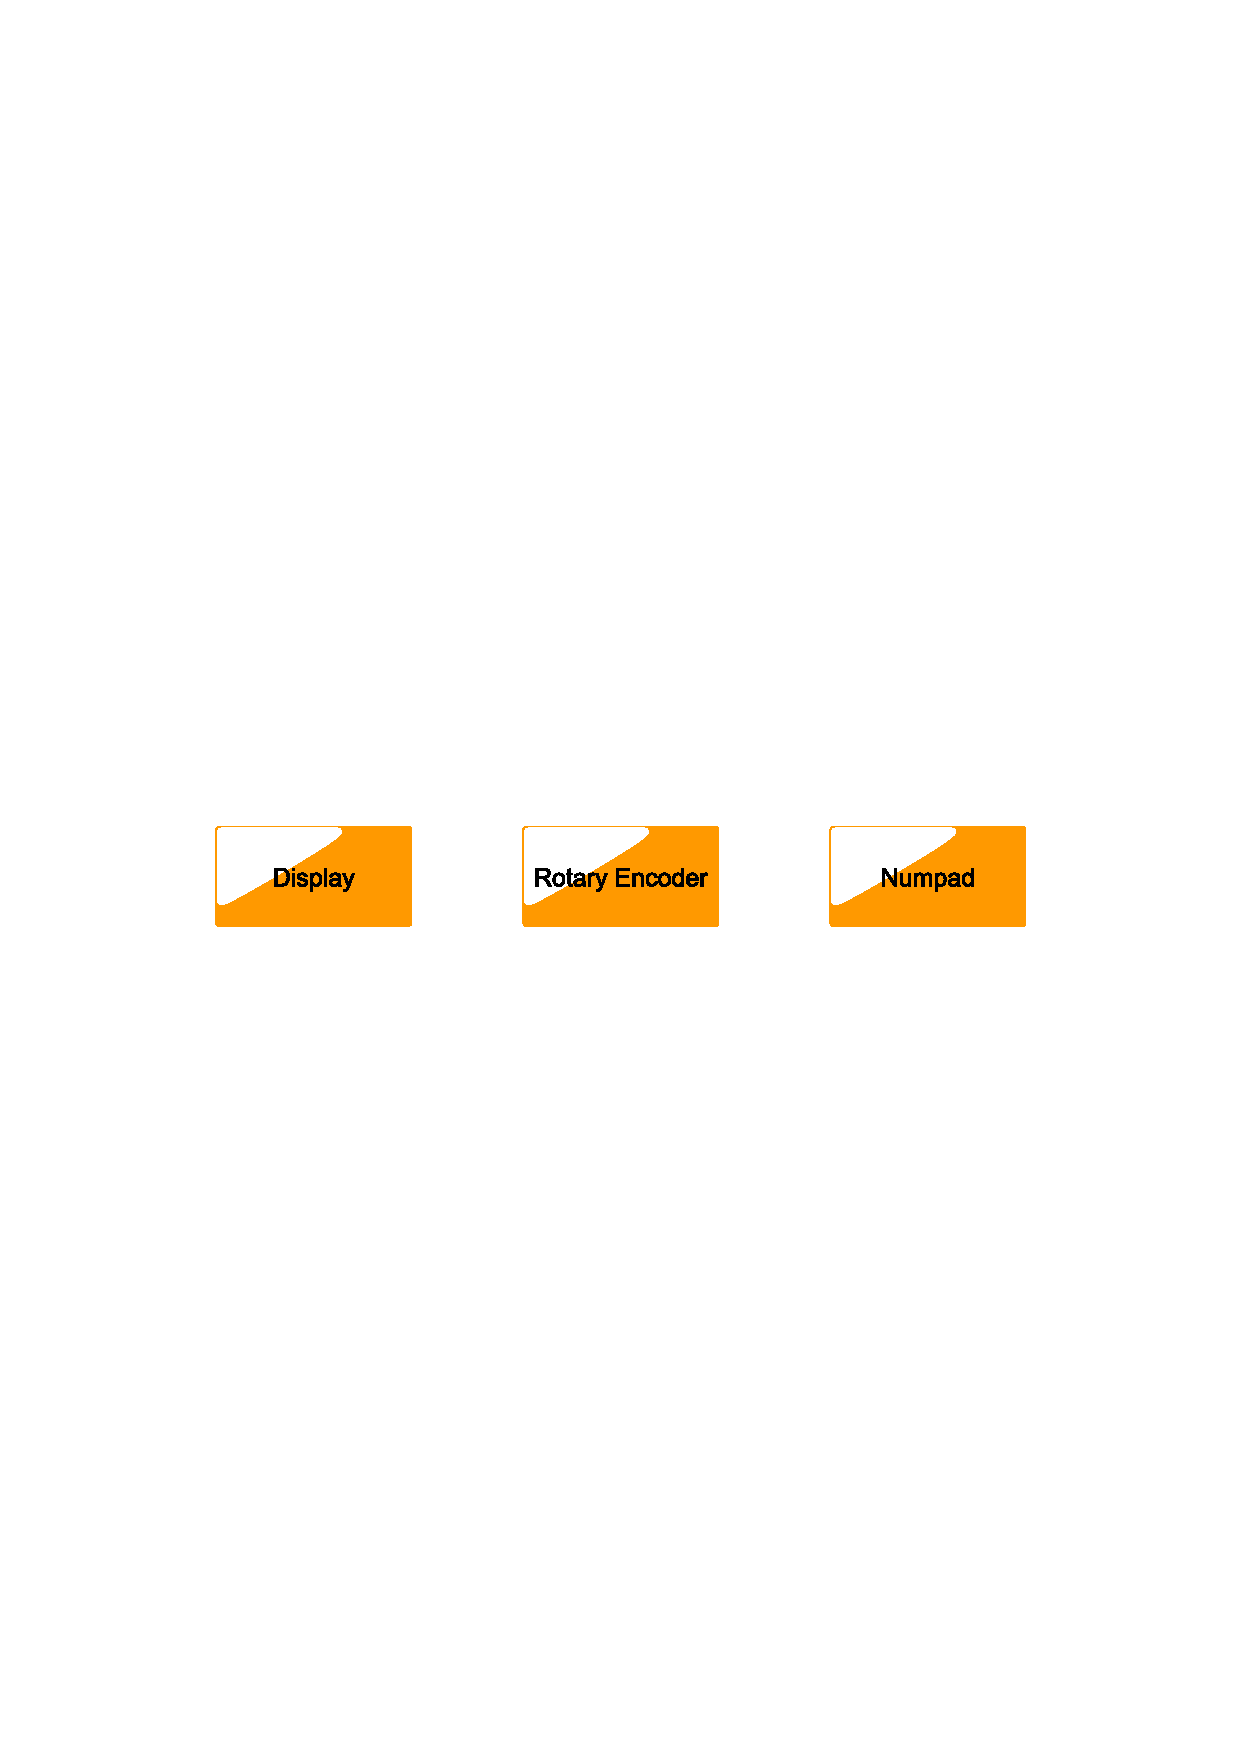
\includegraphics[scale=0.6,clip,trim=00 400 00 400]{graphics/iodevices} %trim=l b r t (can cut off from every side)
	\caption{Set up of the I/O devices.}
	\label{fig:iodevices}			% figure labels are of the form \label{fig:*}
\end{figure}


\section{The complete system}

The electrical system was set up as shown in figure \ref{fig:digitalsystem}. All the user interface mounted with the microprocessor, all the motor input and output at the FPGA and a SPI connection between the two.

\begin{figure}[htb]
	\centering
	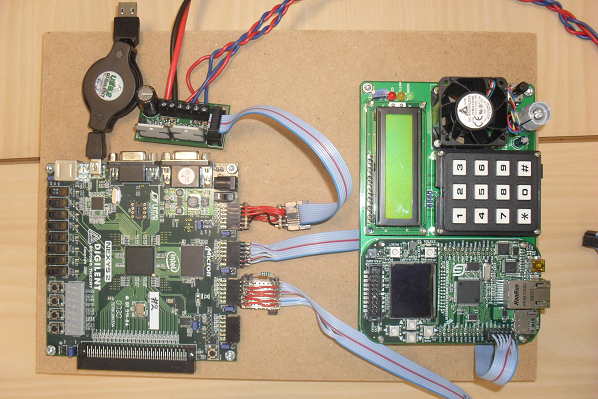
\includegraphics[width=\textwidth]{graphics/digitalsystem.png} %trim=l b r t (can cut off from every side)
	\caption{Set up of the electrical system.}
	\label{fig:digitalsystem}			% figure labels are of the form \label{fig:*}
\end{figure}


The complete system is shown in figure \ref{fig:completesystem}, this shows the parts the system have been divided into. This is not meant to show the exact number of tasks, but as a reference to understand the components in the system.


\begin{figure}[htb]
	\centering
	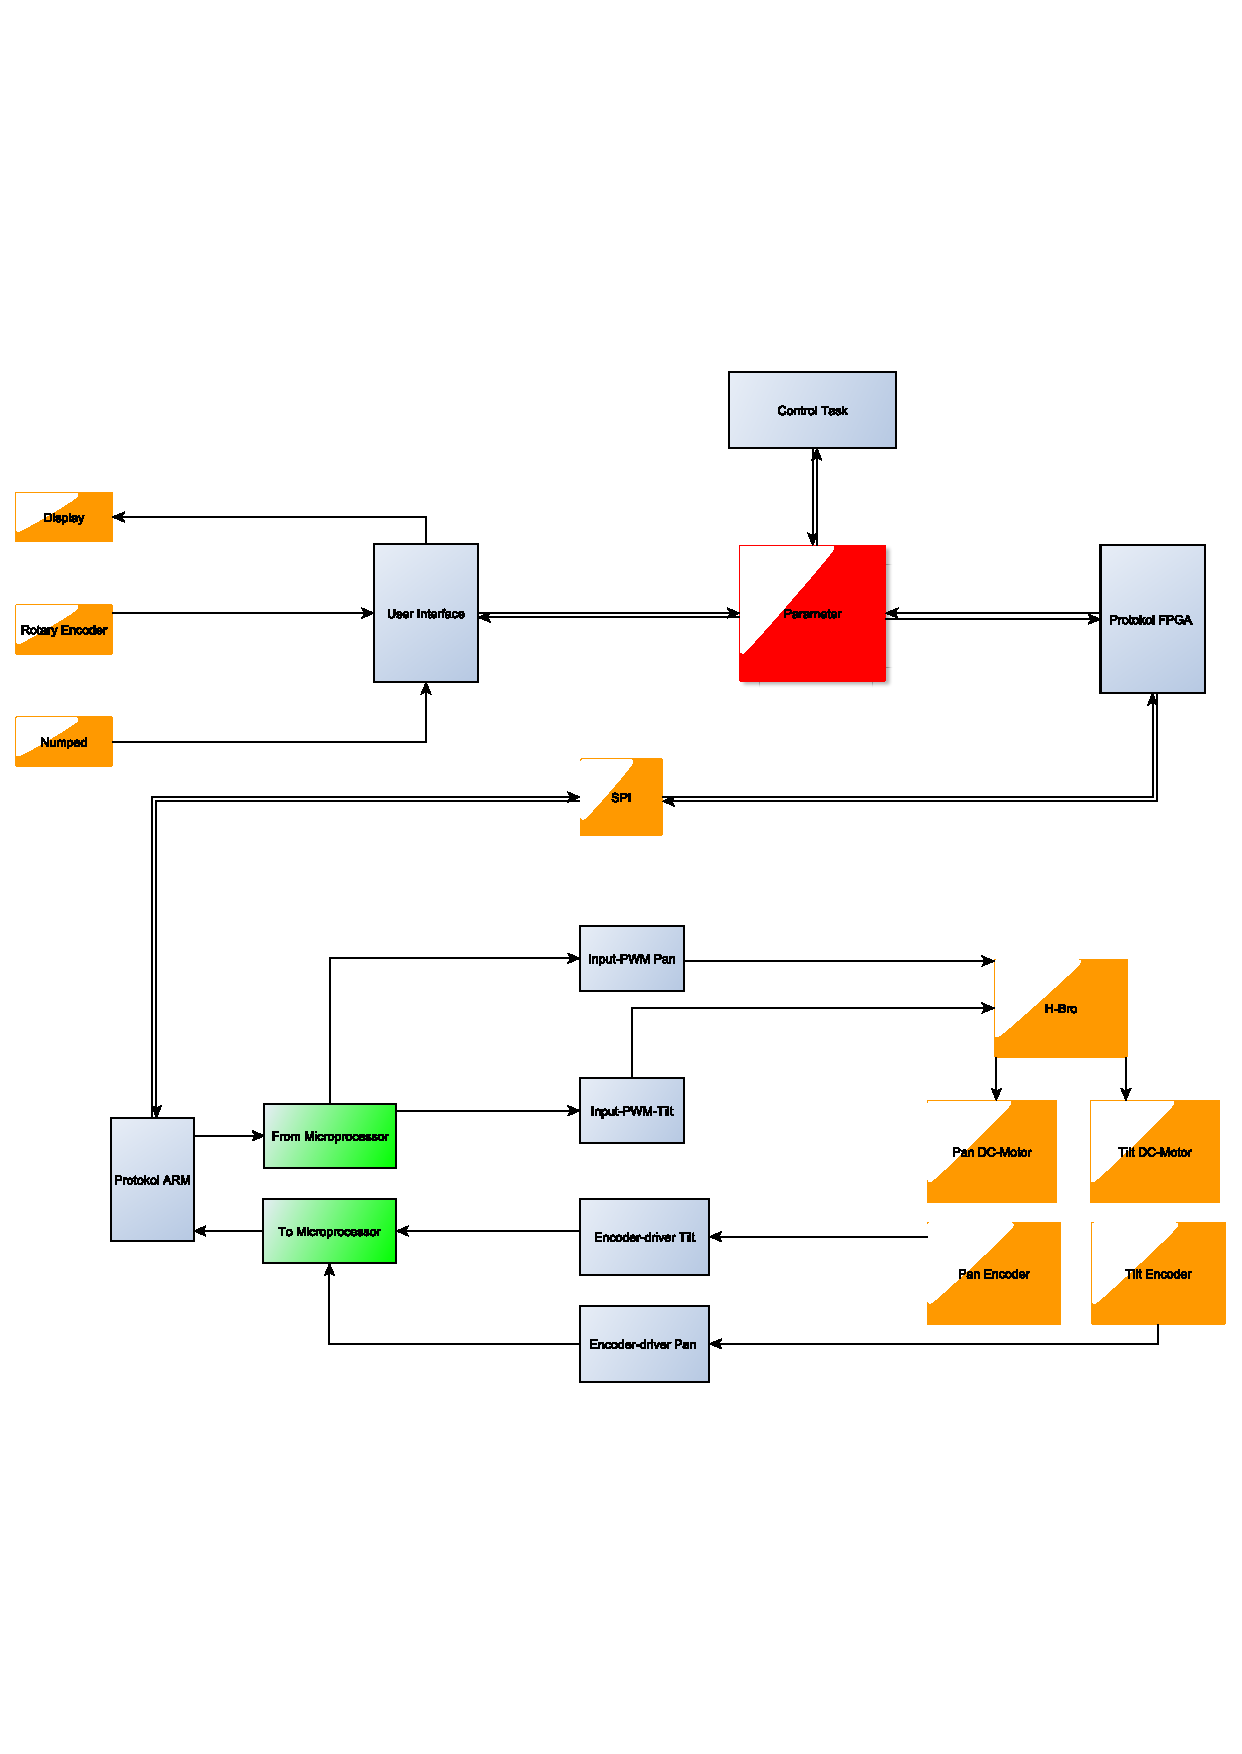
\includegraphics[width=\textwidth,clip,trim=0 160 0 160]{graphics/Project4GreaterPresentation4.pdf} %trim=l b r t 
	\caption{The combined model of parts that the system will consist of. }
	\label{fig:completesystem}			% figure labels are of the form \label{fig:*}
\end{figure}
